% Chapter Template

\chapter{Haskell Type Checking} % Main chapter title

\label{chap:haskell-type-checking}

\graphicspath{{Figures/HaskellTypeChecking}}
In this chapter, we delve into the overview of the technique of type-checking Haskell programs. Haskell uses static types, meaning that type-checking algorithms are run when the user compiles the code. More specifically, this happens after the parsing (as the complete syntax tree is necessary for type checking) and before any low-level code is generated. In a simplistic sense, type checking returns a binary result: the program is type correct or ill-typed. However, as we will see, many interventions have been developed to enrich the type-checking results.

\section{Why Haskell}

The main contribution of my thesis is the theme of developing systems to improve the type debugging experience in Haskell. Despite the fact that we are dedicated to extending our work to other languages, there are important reasons why we implemented these tools for Haskell to begin with.

\subsection{Haskell In Education}

As we mentioned in Chapter \ref{chap:introduction}, teaching programming in undergraduate computer science courses is an important application of Haskell and a primary design goal of the language.  Many textbooks for first-year computer science courses and introduction to functional programming use Haskell as the learning tool \cite{Bird1998-kv, Davie1992-xv}. Although enthusiasts often argue that Haskell is an ideal platform to teach pure function thinking, real-world university adoption appears to be underwhelming. In fact, helping students tackle programming errors in Haskell is a common challenge in teaching Haskell \cite{Jun2000-yu, Tirronen2015-nr}. Some suggest teaching Haskell with a reduced feature set to prevent the frustration of complex type errors \cite{Heeren2003-mz}. Our research is hugely motivated by the drive to realize Haskell's educational value as well as the challenges of teaching Haskell in real life.

\subsection{Haskell In Mathematics and Formal Logic}

Another important application for Haskell is its application in discrete mathematics and formal logic. Because of its strong type system and enforcement of purely functional computation, Haskell has been standing in the middle of general-purpose programming language and proof assistance. Tools like QuickCheck \cite{Claessen2000-rl} have eased the barrier to writing verifiable programs and have since been borrowed to other languages as well. Some proposed using Haskell in hardware verification \cite{Bjesse1998-lh}. However, a common challenge of using these formal systems is its expandability. Our research proposes such an interactive explanation system that allows users to check the development of a proof or refutation step by step, each time with a small amount of mental burden. 


\subsection{Haskell's Relatively Small Language Specification}

Although Haskell's full language semantics were never formally defined \cite{Hudak2007-kn}, it does not stop the language from being studied for programming language innovations, nor does it stop researchers from making meaningful contributions using this language as a platform. Many efforts have been made to formalize subsets of Haskell language \cite{FaxEn2002-nd}. Our research in Haskell benefits from the relatively small language specification, which allows us to quickly implement new ideas and seek feedback.  We also benefit from the welcoming and vibrant Haskell community to help steer our efforts towards correctness and better usability. 


\section{Hindley-Milner Type Inference and Algorithm W}

Type inference, also known as implicit typing, is a technique to reduce the number of occurrences of manually ascribing types. Almost all languages today employ a certain level of type inference. For instance, in Java before 10, a common pattern is that a user must declare a variable with a type, often by writing down the class name, and then initialize the variable, again using the same class name \ref{fig:example-java}. This clearly leads to duplicated knowledge and verbose code. This has been addressed in later versions (Java 10 and later) by using the \texttt{var} keyword \cite{noauthor_undated-an} to declare variables, and the types of the variables can be guessed at compile-time based on the right-hand-side of the assignments.  

\begin{figure}[hbt]
  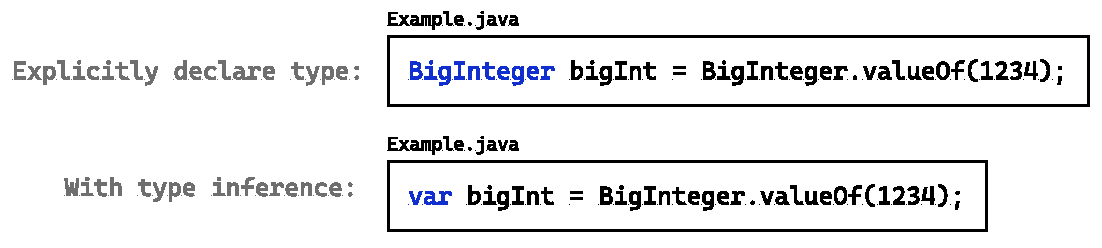
\includegraphics[width=\linewidth]{ExampleJava}
  \caption{
    \label{fig:example-java}
      An example of a typical Java program before and after introducing the \texttt{var} keyword. Before (Top), programmers have to annotate the type identical to the value initializer. After Java 10, this is solved using the local type inference with the \texttt{var} keyword (Bottom).
    }
\end{figure}

In language like Haskell and ML, not only is type inference applied, but its power to detect type error is hugely amplified by the use of the Hindley-Milner type inference. For the example in \ref{fig:example-java}, type inference happens locally within the assignment statement, meaning that the compiler will complain if it cannot gather enough information about the type when analyzing this line. With Hindley-Milner type inference, the compiler will delay making any assertions and continue type-checking the rest of the program. 

The Hindley-Milner Type System \cite{Damas1982-zw} is a foundational part of the type system in many functional programming languages, including ML, Haskell, and Elm. The Hindley-Milner Type System, named after its inventors Roger Hindley and Robin Milner, is a type system that can automatically infer the types of expressions in a language with no annotations required. The system provides polymorphic typing, meaning that a variable can be assigned multiple different types automatically based on its usage context, making it easier to write flexible, reusable code without compromising type safety. In many languages that use this system, it is proven that every expression will be assigned a most general type (principal type) based on its usage. 



\begin{figure}[hbt]
    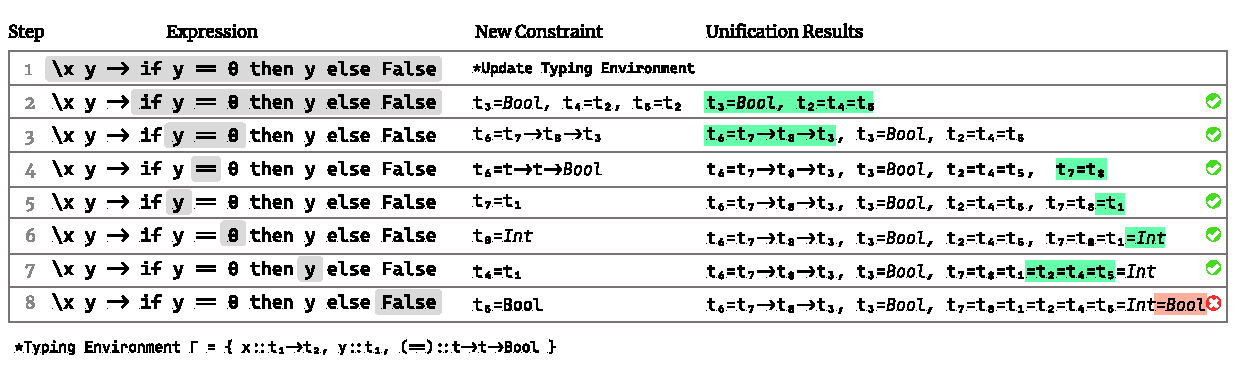
\includegraphics[width=\linewidth]{HindleyMilner}
    \caption{
      \label{fig:hindley-milner}
        An illustration of Hindley Milner Type Checking Performed on a Lambda Expression, \todo{Expand this figure}}
\end{figure}


\textbf{Algorithm W} The original version of the Hindley-Milner type system uses an algorithm -- W -- to identify the most general types for every expression. The algorithm works by first assuming that each expression has a unique type variable associated with it; it recursively inspects the substructure of the program, collecting constraints and applying unification \ref{fig:hindley-milner}. Depend on the type of syntax node, during a step new variables may be created, variables may unify with other variables or concrete types. If at any time the unification step fails, the type-checking stops, and the location from which the last constraint is generated will be reported as the source of the type error.



Despite the seismic influence in type theory, and the conciseness of programming style it helps achieved,  Hindley-Milner type system introduced some setbacks in terms of usability. More specifically, its error message when unable to complete the type inference process leads to confusion among the programmers. 

Because of the way unification is carried out, only one constraint (the last one added) is reported in the type error message, and the other end of the conflict is unable to be retrieved. Unlike in the Java example, where programmers only need to scan the source code for one line, with the Hindley-Milner-based type system, the potential root cause may lie anywhere in the source code.

\textbf{Algorithm M} 
To mitigate the usability issue caused by Algorithm W, others proposed a similar algorithm -- M \cite{Lee1998-fx} -- which, instead of processing type inference bottom-up, carries the outer constraints into the inner structure, achieving a top-down type inference and better error messages in some cases. 

\begin{figure}[hbt]
  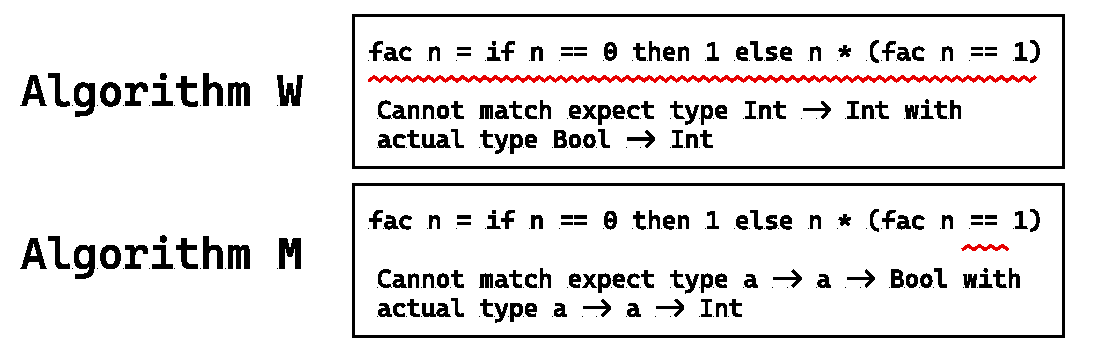
\includegraphics[width=0.8\linewidth]{AlgorithmWM1.pdf}
  \caption{
    \label{fig:algorithm-m-1}
      An example where Algorithm M out-guessed Algorithm W, reporting a more plausible error location.}
\end{figure}


\begin{figure}[hbt]
  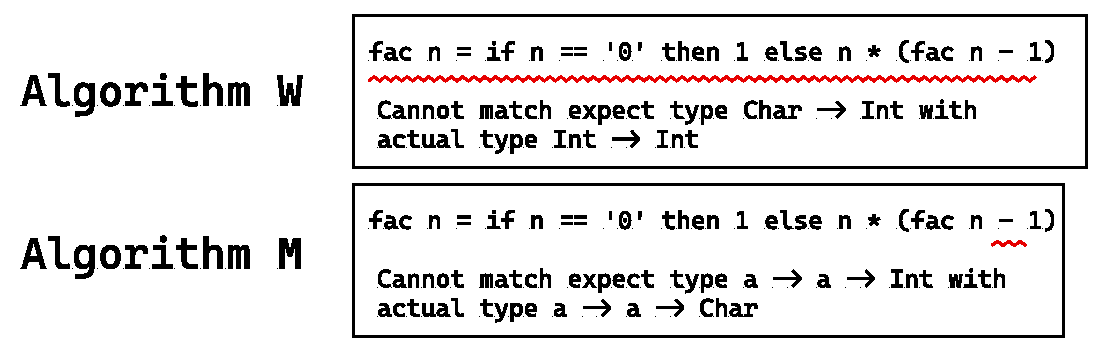
\includegraphics[width=0.8\linewidth]{AlgorithmWM2}
  \caption{
    \label{fig:algorithm-m-2}
    An example where Algorithm M may miss the correct location. It is more plausible here that \texttt{'0'} is a typo.}
\end{figure}


As a result, algorithm M is able to identify certain errors more accurately than algorithm W \ref{fig:algorithm-m-1}. However, it is equally misleading in some other cases \ref{fig:algorithm-m-2}. An important lesson that can be learned from these approaches to type inference is that no method ensures that the result will match the programmers' true intention. At its core, algorithm M and algorithm W suffer from the same issue: the unification is done one step at a time, and the earlier constraints are discarded once they are successfully unified. Rather than ambitiously pinpointing where the root cause may lie, a more realistic goal might be to represent type errors succinctly without making assumptions.



\section{Type Error Slicing}

Type error slicing \cite{Tip2001-qn, Haack2004-fr} is a technique that aims to represent type error by including more useful information for the programmers. Compared to the Hindley-Milner approach, it relies on delaying the unification until all constraints are generated. Two important ideas have been employed in type error slicing: 


\begin{enumerate}
  \item {
    Labeled constraints. Assign constraints to locations in programs, and these locations are later retrieved and identified as part of the error diagnosis. 
  }
  \item {
    Minimal unsatisfiability analysis. Finding the minimal unsatisfiable locations that contributed to a type error  as a standard process of type error diagnosis. In practice minimal unsatisfiable locations avoid being too general as in algorithm W, and avoids being too biased as in both algorithm W and algorithm M. 
  }
\end{enumerate}


\begin{figure}[hbt]
  \includegraphics[width=0.5\linewidth]{TypeErrorSlicing.pdf}
  \caption{
    \label{fig:type-error-slicing}
      An example of type error slicing}
\end{figure}

Compared to traditional tools, type error slicing shows complete error locations \ref{fig:type-error-slicing}, and programmers are able to reason about the type error because both sides of the typing conflict are included. 

Over the years, type error slicing has become the go-to approach for optimizing type errors. Many have improved and generalized the method of producing minimal, unsatisfiable locations. The process generally involves removing constraints one at a time and checking the feasibility of the system changes. Different underlying constraint languages have been studied to encode more advanced type system features. This includes using SMT \cite{Pavlinovic2015-ke} and Constraint Handling Rules \cite{Stuckey2003-pz}. 



\section{Interactive Type Debugging}

In conventional program slicing approaches, a Minimal Unsatisfiable Subset (MUS) is typically used to represent a single type error, thereby providing a comprehensive set of locations. However, we have identified two significant limitations inherent in MUS-based localization and diagnosis:

\begin{figure}[hbt]
  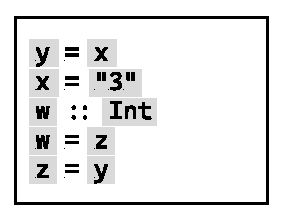
\includegraphics[width=0.5\linewidth]{SlicingCounterExample}
  \caption{
    \label{fig:slicing-counter-example}
      An example where type error slicing essentially highlights every location in the program.}
\end{figure}

MUS-based error slicing can narrow down the potential defected locations to some extent. However, research indicates that program slicing can only reduce around 30\% of the code size that is required to understand a type error \cite{binkley_empirical_2007}. Further reduction is challenging with the knowledge of MUS alone due to the MUS's minimality. For instance, in the code shown in \ref{fig:slicing-counter-example}, type error slicing essentially highlights every location in the program. Clearly, there is more important information that needs to be encoded in the type error.

Chameleon \cite{Stuckey2003-pz} is a project that was created as a command-line tool in the early 2000s to improve type error reporting 
for the Haskell programming language. Like other type-error slicing approaches, Chameleon used a more general constraint language -- CHR -- which in turn allows more flexible constraint relations to be defined in the constraint language. This is signified by the successful support of advanced type-level features such as type class and functional dependencies. More importantly, Chameleon employed the notion of interactive type debugging. In the example, Chameleon not only highlighted all the relevant locations but also reflects the fact that two sets of potential types (most general unifiers) can be found in the ill-typed program, and they can be traced back to two sets of locations in the source code. Programmers can proceed to query the type information of either potential resolution as if the type error has been resolved.


\begin{figure}[hbt]
  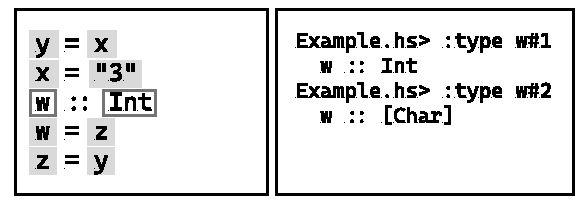
\includegraphics[width=0.8\linewidth]{ChameleonInteractive}
  \caption{
    \label{fig:chameleon-interactive}
      An example where type error slicing essentially highlights every location in the program.}
\end{figure}

\section{The Analysis Of An Unsatisfiable System}

One advantage of using a slicing-based approach is that many tools are available from the study of constraint satisfiability. Among them, a few important ones are the Minimal Unsatisfiable Subset (MUS), Minimal Correction Subset (MCS), and Maximal Satisfied Subset (MSS).  

\subsection{Minimal Unsatisfiable Subset}

MUS is the most commonly used tool in programming error analysis. Most program slicing-based tools \cite{Haack2004-fr, Pavlinovic2015-ke, Stuckey2003-pz} use MUS one way or another. Intuitively, MUS is the smallest subset of a constraints system that still remains infeasible. Infeasibility here simply means there are no ways to assign value to the logical variables. For an ill-typed program, this means finding a minimal set of locations that can explain the logical conflict of a type error. 

Formally,  a minimal unsatisfiable subset (MUS) $M$ of a constraint system $C$ is a subset $M \subseteq C$ such that $M$ is unsatisfiable and $ \forall{c} \in M : M \setminus \{c\}$ is satisfiable. An MUS can be seen as a minimal explanation of the infeasibility of the constraint system. MUSes have been used extensively, mostly in combination with programming slicing, as a means to explain type errors. A MUS of type system constraints encodes a path of reasoning connecting all evidence from one location of the conflict to another.


It needs to be made clear that, for a constraint system, multiple MUSes may exist. In the example in Fig \ref{fig:mus-example}, the constraint system contains 5 propositional constraints. Clearly, the whole system is infeasible. However, there are 3 possible MUSes in this system. We know that each MUS is minimal because removing any single constraint from a MUS will make it satisfiable. Conventionally, we use a shrink-based algorithm to find the MUS set. The basic idea is removing one constraint a time from the constraint set, until the remaining subset is satisfilbe. In this case, the last removed item must be a subset of MUS. And thus repeating the process until a MUS is derived. Although finding such a subset can be computationally expensive, it is useful because it represents the type error with comprehensive reasoning of how the error is inferred.


\begin{figure}[hbt]
  \includegraphics[width=0.8\linewidth]{MUS}
  \caption{
    \label{fig:mus-example}
      An example of possible MUSes of a constraint system in propositional logic}
\end{figure}

\subsection{Minimal Correction Subset and Maximally Satisfiable Subset}

Despite its wide usage in type inference, MUS is not the only useful subset for representing type error. Minimal correction subset (MCS) can be understood as the smallest subset that needs to be removed to make the rest of the system satisfiable. Formally, a minimal correction set (MCS) $M$ of a constraint system $C$ is a subset $M \subseteq C$ such that $C \setminus M$ is satisfiable and $\forall{S} \subset M : C \setminus S$ is unsatisfiable. MCSes are so named because their removal from $C$ can be seen to “correct” the infeasibility. Because of the property that ``Removing MCS will repair the rest of the system", MCS is effective in representing the cause of the error. In an ill-typed program, an MCS can be seen as the smallest set of locations that need to be modified to fully resolve the type error.  Like a constraint system, which can have multiple MUSes, MCSes are not unique either. In the example (Fig. \ref{fig:mcs-example}), 4 MCSes can be found. Removing each of these will result in a satisfiable set of constraints. 

\begin{figure}[hbt]
  \includegraphics[width=0.8\linewidth]{MCS}
  \caption{
    \label{fig:mcs-example}
      An example of possible MCSes of a constraint system in propositional logic}
\end{figure}

The Maximal Satisfiable Subset is the complement of MCS. Formally, a maximal satisfiable subset (MSS) $M$ of a constraint system $C$ is a subset $M \subseteq C$ such that M is satisfiable and $\forall{c}\ in\ C \setminus M:M\cup\{c\}$ is unsatisfiable. The definition of an MSS is symmetric to that of a MUS, with `satisfiable' and `unsatisfiable' swapped along with maximal for minimal. In an ill-typed program, an MSS can be seen as the resulting typing environment if a type error is fixed by relaxing the MCS. An example of MSSes in a constraint system can be seen in Fig \ref{fig:mss-example}.


\begin{figure}[hbt]
  \includegraphics[width=0.8\linewidth]{MSS}
  \caption{
    \label{fig:mss-example}
      An example of possible MSSes of a constraint system in propositional logic}
\end{figure}1

\subsection{MUS Enumeration}
 Minimal Unsatisfiable Subsets are often not unique, so it is possible for an unfeasible system to contain a finite number of MUSs. In practice, the existence of multiple MUSes itself is a valuable piece of information. In type checking, it indicates that there are multiple sources of conflict. Enumerating multiple MUS/MCS, in this case, provides better insights into the root cause and how to address them properly. We will present an application of enumerating MUS/MCS in Chapter \ref{chap:goanna}.

The problem with MUS enumeration is that it is computationally expensive. In the most naive approach, it requires exploring the power set of all constraints in the constraint system. In fact, most of the effective enumeration algorithms today rely on heuristics, and they provide performance improvements on a case-by-case basis. MARCO~\cite{Liffiton2016-xi} and MUST~\cite{Bendik2020-pz} are examples of such an approach. They use heuristics to avoid traversing a large chunk of the subsets, each representing a permutation of which constraints need to be relaxed and which do not.


% \begin{figure}[hbt]
%   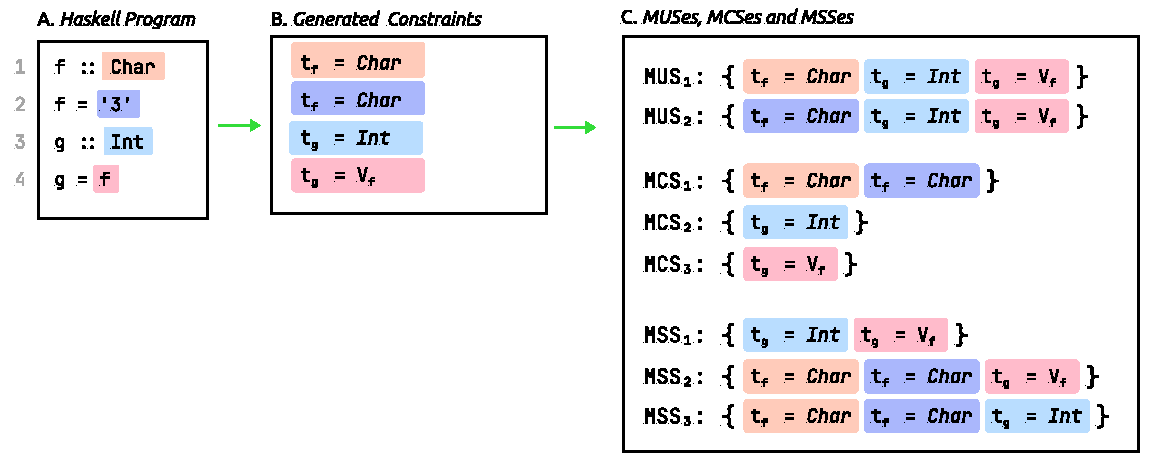
\includegraphics[width=\linewidth]{Subsets}
%   \caption{An example of generating constraints from Haskell program, and all the possible MUSes, MCSes, and MSSes can be acquired.}
% \end{figure}

\section{Three Classes of Type Error}
With the introduction of MUS, we can revisit the idea of three categories of type error we proposed in Chapter \ref{chap:introduction}. This categorization allows a formal study of the tools that are necessary to cover the information of a given type error. 

\subsection{Multi-step Type Error}
\begin{figure}[hbt]

  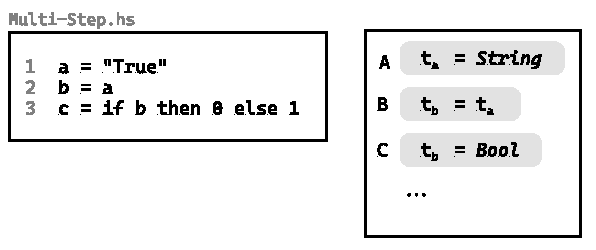
\includegraphics[width=0.5\linewidth]{Multi-Step-2}
  \caption{
    \label{fig:multi-step-2}
    A multi-step type error
  }
\end{figure}
Multiple-step type errors contain a chain of reasoning steps or a series of attempts to unify two logical terms. Multiple-step type error contains a single MUS. Each element of the MUS forms a singleton MCS. In the example of Fig \ref{fig:multi-step-2}, the MUS is the set of {A, B, C}. The MCSes are {A}, {B}, {C}. Removing any one of the MCSs will result in the program type check.

\subsection{Multi-witness Type Error}
\begin{figure}[hbt]
  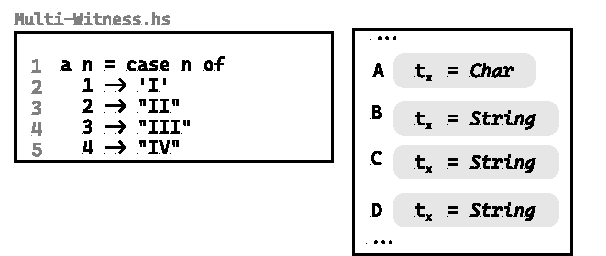
\includegraphics[width=0.5\linewidth]{Multi-Witness-2}
  \caption{
    \label{fig:multi-witness-2}
    A multi-witness type error
  }
\end{figure}

A Multiple-witness type error occurs when one side of the conflict contains multiple locations (witnesses) suggesting the same typing assignment. If one such location is removed, the type error will remain. In the example (\ref{fig:multi-witness-2}), there are three MUSes: {A, B}, {A, C}, {A, D}. Therefore, this type of error cannot be succinctly represented by a single MUS. 

\subsection{Multi-party Type Error}
\begin{figure}[hbt]
  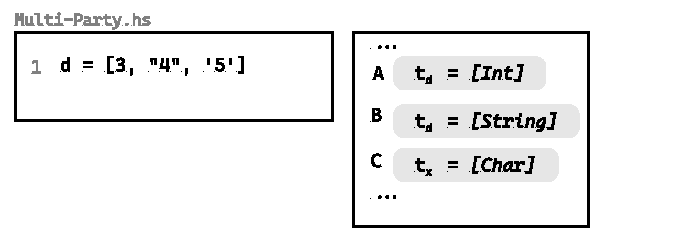
\includegraphics[width=0.5\linewidth]{Multi-Party-2}
  \caption{
    \label{fig:multi-party-2}
    A multi-party type error
  }
\end{figure}

A multiple-party type error is an error where multiple types of irreconcilable assignments can be obtained from locations in the source code. In the provided example  (\ref{fig:multi-party-2}), there are 3 MUS: {A, B}, {A,C}, {B,C}. Therefore, this type of error cannot be succinctly represented by a single MUS.

\begin{figure}[hbt]
  
  \includegraphics[width=\linewidth]{Compare}
  \caption{}
\end{figure}

\section{Conclusion}
In this chapter, we established a subset of the Haskell language by defining its syntax and typing rules. We explored two avenues to type-check a program in such language and obtain principle types: using the Hindley-Milner type system and using a constraint-based type system. In addition, we explored some type error analysis tools that are enabled by using a constraint-based type system and how these tools are applied to three different kinds of type errors. We will explore them in the next two chapters.
